\documentclass{article}

\usepackage{graphicx}

\begin{document}

\begin{figure}
  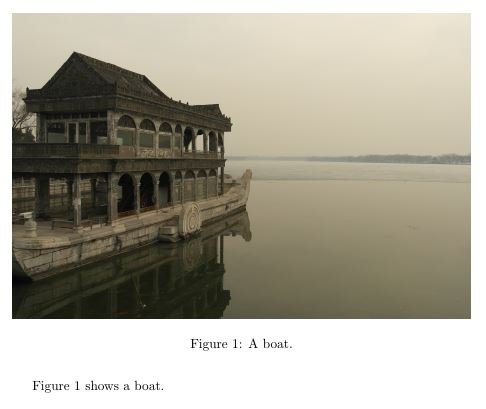
\includegraphics[width=\linewidth]{boat.jpg}
  \caption{Two boat.}
  \label{fig:boat1}
\end{figure}
This is some example text\footnote{\label{myfootnote}Hello footnote}.

Figure \ref{fig:boat1} shows a boat.
I'm referring to footnote\ref{myfootnote}.


\begin{table}[h!]
  \centering
  \caption{Caption for the table.}
  \label{tab:table1}
  \begin{tabular}{l|c||r}
    1 & 2 & 3\\
    \hline
    a & b & c\\
  \end{tabular}
\end{table}

\section{section 1}


\begin{table}[h!]
\centering
\caption{Caption for the table.}
  \label{tab:table1}
  \begin{tabular}{ccc}
%  \toprule
    Some & actual & content\\
%    \midrule
    prettifies & the & content\\
    as & well & as\\
    using & the & booktabs package\\
%    \bottomrule
  \end{tabular}
\end{table}




\end{document}
